\documentclass{article}

\title{\textbf{Gaseous detectors and GEMs} }
\author{Sebastián Montoya Hernández}


\usepackage[english]{babel}
\usepackage{graphicx}
\usepackage{amsmath}
\usepackage{cite}
\usepackage{hyperref}
\usepackage{caption}
\usepackage{float}
\usepackage{listings}



\begin{document}

\maketitle 
\setcounter{section}{0}
Aquí va la introducción del capítulo
\newpage
\section{Marco teórico}

Aquí va la introducción del marco teórico, mencionando en orden todas las subsecciones.

En numerosos experimentos de física de partículas, los detectores gaseosos, incluidos los GEMs, desempeñan un papel crucial en la medición de partículas cargadas mediante la ionización de gases. Estos detectores permiten trazar con precisión las trayectorias de las partículas, especialmente en entornos con campos magnéticos. En comparación con los detectores de semiconductores, los detectores gaseosos suelen ser más económicos, especialmente en aplicaciones que requieren cubrir grandes volúmenes, y presentan menos material que pueda interferir con las partículas que atraviesan el detector \cite{sauli2015gaseous}. Dado que los detectores GEM son el enfoque principal de este trabajo, en el presente capítulo se explorarán los conceptos fundamentales de la física que rigen sus interacciones y funcionamiento.

\subsection{Principios físicos de los detectores gaseosos}

\noindent En términos generales, la detección de una partícula se logra mediante la deposición de una fracción o la totalidad de su energía en el medio con el que interactúa. Aunque fenómenos como la luminiscencia o la emisión de fotones de centelleo, entre otros, pueden manifestarse como resultado de la interacción entre partículas cargadas o fotones y medios gaseosos, la ionización es la interacción predominante en sistemas de baja densidad, y puede aprovecharse para generar una señal medible. En el proceso de ionización de un gas, la energía de la partícula incidente excita los electrones de las capas externas de los átomos, liberándolos y formando pares ion-electrón en su recorrido. Estos electrones iniciales pueden continuar interactuando con el medio, provocando nuevas ionizaciones y excitaciones. En materiales compuestos, los procesos secundarios también contribuyen al número total de electrones generados, ya que parte de la energía de excitación se transforma en ionización o viceversa. Aunque los detectores gaseosos se centran principalmente en la captación de los electrones liberados por la radiación ionizante, la presencia de iones, estados excitados o fotones puede desencadenar fenómenos secundarios, como recombinación, transferencia de carga y efectos fotoeléctricos. En la figura \ref{fig:ionization_chamber1}, se ilustra la estructura básica de un detector gaseoso.

\begin{figure}[H]
    \centering
    \includegraphics[width=1.0\textwidth]{ionization_chamber.PNG}
    \caption{Diagrama que describe el funcionamiento básico de un detector gaseoso. El medio sensible del detector, en este caso un gas, se encuentra entre dos electrodos con un voltaje aplicado. Cuando una partícula cargada atraviesa el gas, se liberan cargas que se desplazan hacia los electrodos impulsadas por el campo eléctrico. Estas cargas en movimiento generan una señal de corriente en los electrodos. En esencia, el detector actúa como un condensador que se descarga cuando el medio es ionizado. Desde el punto de vista eléctrico, se comporta como una fuente de corriente.}
    \label{fig:ionization_chamber1}
\end{figure}

\noindent Si los eventos de ionización en un gas son estudiados de manera independiente en este contexto, es posible realizar una descripción que sigue la estadística de Poisson

\begin{equation}
    \label{eq:poisson}
    P_k^n=\frac{n^k}{k!} \mathrm{e}^{-n}
\end{equation}

\noindent donde $ P_k^n$ es la probabilidad de observar $k$ eventos en un intervalo fijo, dado un promedio o tasa de eventos $n$. Por definición, se asume que los eventos son independientes: la ocurrencia de uno no afecta la probabilidad de los demás. De esta manera, la eficiencia teórica del detector, entendida como la probabilidad de tener al menos una interacción, es entonces

\begin{equation}
    \label{eq:det_eff}
    \varepsilon=1-P_0^n=1-\mathrm{e}^{-n} .
\end{equation}

\noindent Debido a que no existe una expresión simple para determinar el número de encuentros ionizantes primarios, es necesario recurrir a datos obtenidos experimentalmente o a programas de simulación especializados. Si no se tienen en cuenta procesos secundarios como la recombinación, por ejemplo, siendo $\Delta E$ la energía depositada en el medio y $W_{I}$ la energía por par íonico, la cantidad total de pares iónicos en el medio puede ser calculada como 
\begin{equation}
    \label{eq:num_ion}
    N_{T} = \frac{\Delta E}{W_{I}}.
\end{equation}

\noindent No obstante, este es un resultado promedio. Para entender con detalle la distribución energética en este fenómeno, es necesario acudir a un marco teórico más robusto. La pérdida de energía cinética de la partícula a medida que avanza por el volumen del detector es conocida como stopping power o ecuación de Bethe-Bloch y una formulación semiclásica para calcularla en un medio de grosor $\Delta x$ es: 

\begin{equation}
    \label{eq:bethe_bloch}
    \frac{\Delta E}{\Delta x}=-\rho \frac{2 K Z}{A \beta^2}\left[\ln \frac{2 m c^2 \beta^2}{I\left(1-\beta^2\right)}-\beta^2-\frac{C}{Z}-\frac{\delta}{2}\right], \quad K = \frac{2 \pi N e^{4}}{mc^{2}}
    \end{equation}

\noindent donde $\beta$ es la velocidad de la partícula, $m$ y $e$ son la masa y la carga del electrón, $Z$, $A$ y $\rho$ son el número atómico, masa atómica y la densidad del medio, $I$ es el potencial promedio de ionización del medio, el término $C/Z$ hace referencia a correcciones por apantallamiento con capas electrónicas internas y $\delta /2$ solo tiene relevancia en el régimen relativista. Para estimar las mencionadas correcciones, es necesario acudir a tablas de referencia o hallar los parámetros a partir de ajustes con datos experimentales.\\ 

\noindent Algunas consideraciones que deben ser tenidas en cuenta respecto a la ecuación de Bethe-Bloch, son su aplicabilidad a medios isotrópicos, debido a la aparición de "channeling effects" en sistemas cristalinos y las excepción de electrones y protones como partículas incidentes por su indistinguibilidad en la materia [2].\\

\noindent Teniendo en cuenta que la velocidad de la partícula ionizante es uno de los parámetros que rigue la ecuación \ref{eq:bethe_bloch}, es posible describir el comportamiento de su pérdida de energía para distintos regímenes de velocidad como ilustra la figura \ref{fig:bethe_b} [3].

\begin{figure}[H]
    \centering
    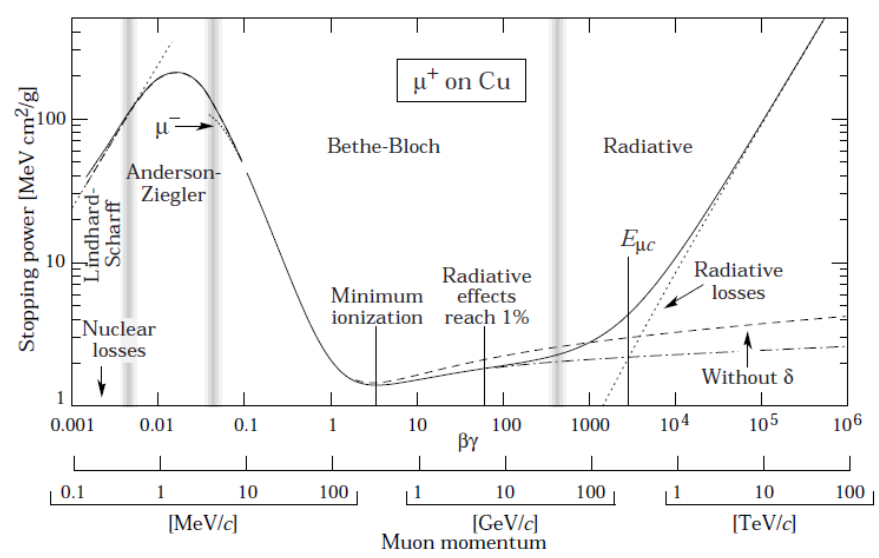
\includegraphics[width=0.8\textwidth]{bethe_bloch.PNG}
    \caption{La fórmula de Bethe-Bloch para muones positivos en cobre como función de la velocidad [3] (mostrada entre la segunda y tercera banda gris. El resto se describe mediante otros modelos).}
    \label{fig:bethe_b}

\end{figure}

\noindent Los iones y electrones generados por procesos ionizantes en un gas pierden rápidamente su energía mediante sucesivas colisiones con las moléculas del entorno, equilibrándose con la energía térmica del medio. Al ser sometidos a campos coulombianos en el medio, las cargas se desplazan a través del gas mientras se difunden, hasta que finalmente se neutralizan, ya sea por recombinación en el propio gas o al alcanzar las paredes del recipiente. En el caso de los iones, pueden transferir su carga a otra molécula del mismo gas o a una de diferente tipo con un potencial de ionización más bajo. Los electrones, por otro lado, pueden ser neutralizados al combinarse con un ion positivo, adherirse a moléculas con afinidad electrónica o ser absorbidos por las paredes del contenedor [Loeb, 1961].\\

\noindent No obstante, a pesar de que los electrones se desplazan de forma aleatoria debido a estas interacciones con el medio, en presencia de un campo eléctrico externo, se introduce una tendencia en su desplazamiento denominado deriva electrónica. La velocidad promedio que los electrones alcanzan en su desplazamiento bajo la influencia del campo eléctrico se denomina velocidad de deriva $w^{-}$ y se define como 
\begin{equation}
    w^{-} = \mu E
\end{equation}

\noindent siendo $\mu$ la movilidad electrónica y $E$ la intensidad del campo eléctrico. Según un enfoque simple propuesto por Townsend en 1947, la velocidad de deriva de los electrones puede expresarse mediante 
\begin{equation}
    w^{-}=k \frac{e E}{m} \tau,
\end{equation}

\noindent Aunque esta formulación resulta útil para análisis cualitativos, su aplicación práctica es limitada, ya que los valores de la velocidad de deriva $w$ y el tiempo medio entre colisiones $\tau$ dependen tanto del tipo de gas como de la intensidad del campo eléctrico. Durante su desplazamiento en presencia del campo, los electrones sufren múltiples colisiones con las moléculas, lo que provoca la difusión de la nube de carga inicial. La extensión de esta difusión depende no solo del tipo de gas, sino también de la magnitud del campo eléctrico $E$, ya que un campo más intenso permite que los electrones ganen más energía entre colisiones. De acuerdo a la teoría de transporte de carga basada en principios de mecánica estadística, es posible obtener la relación entre la movilidad electrónica $\mu$ y el coeficiente de difusión $D$, también conocida como fórmula de Nernst–Townsend
\begin{equation}
    \frac{D}{\mu}=\frac{\varepsilon_k}{e}
\end{equation}
\noindent donde $D$ mide la tasa de dispersión de partículas en un medio debido a movimientos aleatorios y $\varepsilon_k$ es una cantidad fenomenológica denominada energía característica, que en el caso particular de difusión térmica toma el valor de $k_{B} T$.\\

\noindent Teniendo en cuenta esto, un importante resultado de la teoría de transporte, que se deriva al considerar una distribución normal localizada de la difusión de los electrones es la expresión de su desviación estándar $\sigma_x$, que describe la extensión de la nube de electrones alrededor de un punto central a medida que se mueven a través del medio bajo la influencia del campo eléctrico aplicado.
\begin{equation}
    \sigma_x=\sqrt{\frac{2 \varepsilon_k}{e} \frac{x}{E}}
\end{equation}

\noindent Esta expresión, también llamada espacio de difusión, no depende por tanto de la presión, solamente de la intensidad del campo eléctrico.\\

\noindent A medida que el campo eléctrico se incrementa, aumenta la probabilidad de colisiones ionizantes y disminuye la de excitaciones. Cada colisión ionizante crea un par electrón-ion, y el electrón primario sigue desplazándose en el gas. Si la trayectoria libre media para colisiones ionizantes es pequeña en comparación con el grosor de la capa de gas, los electrones rápidamente obtienen más energía del campo para continuar ionizando. Esto genera un crecimiento acelerado de una avalancha de electrones e iones, el mecanismo principal para amplificar señales en los contadores proporcionales de gas. Sin embargo, tras una colisión, un electrón puede transferir una cantidad de energía igual o superior a la necesaria para excitar un átomo o molécula. Luego, estos regresan al estado fundamental mediante una o varias transiciones: por ejemplo, los gases nobles emiten fotones al desexcitarse, mientras que las moléculas poliatómicas, como los hidrocarburos, disipan la energía a través de transiciones rotacionales y vibracionales sin emisión de radiación.\\

\noindent Cuando la energía de un electrón acelerado por un campo eléctrico supera el potencial de ionización de un átomo o molécula, los electrones enlazados pueden ser expulsados, dejando atrás un ion positivo. En función de la energía transferida y de la densidad de carga, pueden generarse estados de ionización múltiple. Sin embargo, en las condiciones típicas de los contadores proporcionales, donde las energías de los electrones se mantienen por debajo de unas pocas decenas de electronvoltios (eV), es más común que se formen iones con una sola carga positiva. Si los electrones primarios o secundarios no son capturados o absorbidos por las paredes del detector, continuarán moviéndose a través del gas y podrán generar nuevas ionizaciones. La trayectoria libre media para la ionización ($\lambda$) se define como la distancia promedio que recorre un electrón antes de experimentar una colisión ionizante. El inverso de esta distancia, $\alpha = \lambda ^{-1}$, se conoce como el primer coeficiente de Townsend, y representa el número de pares iónicos generados por unidad de longitud durante el desplazamiento del electrón. Este coeficiente se relaciona con la sección eficaz de ionización (probabilidad de que ocurra una ionización) mediante la expresión 
\begin{equation}
    \alpha=N \sigma_{\mathrm{i}}
\end{equation}

\noindent siendo $N$ el número de moléculas por unidad de volumen. Este mecanismo es clave para la amplificación de señales en detectores gaseosos, ya que cada colisión contribuye a la creación de más portadores de carga, permitiendo detectar eventos con mayor precisión.\\

\noindent El proceso de ionización sucesiva por colisiones permite la amplificación de carga en los contadores proporcionales. Imaginemos un electrón que se libera en una región con un campo eléctrico uniforme. Tras recorrer una trayectoria libre media $1/\alpha$, se produce un par electrón-ion. Ambos electrones continúan su desplazamiento en el gas, generando nuevos pares tras otra trayectoria libre media, y así sucesivamente. Si $n$ representa el número de electrones en una posición dada, su incremento luego de recorrer una distancia diferencial $dx$ es $dn = n \alpha dx$. Al integrar esta expresión sobre una distancia total $x$, se obtiene:

\begin{equation}
n = n_0 e^{\alpha x} \quad \text{o} \quad M = \frac{n}{n_0} = e^{\alpha x},
\label{eq:multiplication}
\end{equation}

\noindent donde \(n_0\) es el número inicial de electrones y \(M\) es el factor de multiplicación o ganancia, que indica la amplificación total de carga. Esta expresión describe cómo el número de electrones crece exponencialmente con la distancia recorrida en el gas, siempre que las condiciones de ionización se mantengan constantes.\\

\noindent Para obtener una lectura precisa de la señal, se puede integrar la corriente a lo largo del tiempo, lo que permite calcular la carga total generada en el detector. La variación del voltaje registrada está relacionada con su capacitancia, y una resistencia externa se utiliza para asegurar que la carga se integre correctamente y la señal se lea con precisión. Aunque las cargas inducidas no dependen de las cargas de polarización del material, la capacitancia del sistema juega un papel crucial en la interpretación correcta de la señal medida.\\

\noindent La corriente inducida por estos electrones en avalancha aumenta con el tiempo y depende de la velocidad de deriva de los electrones y el coeficiente de Townsend. La señal rápida resultante en un contador de avalancha es una fracción de la carga total generada, destacando que al final del proceso de recolección la carga inducida total es proporcional a la carga inicial multiplicada por un factor exponencial. En la figura \ref{fig:avalanche_signal} se observan las corrientes inducidas por la contribución de los electrones e iones en la avalancha para una configuración con parámetros típicos (page 174).

\begin{figure}[H]
    \centering
    \includegraphics[width=0.8\textwidth]{avalanche_signal.png}
    \caption{Corriente inducida por avalancha en cátodos por electrones e iones.}
    \label{fig:avalanche_signal}
\end{figure}

\noindent No obstante, en el caso de una distribución extendida de carga dentro del espacio entre los electrodos, aplica el análisis que llevó a la ecuación \ref{eq:bethe_bloch}. La señal resultante depende de la densidad y distribución espacial de las cargas liberadas en el gas. En el caso particular de una ionización uniforme entre ánodo y cátodo, con una densidad \( \rho \), siendo $T$ el tiempo total de colección para los electrones en la avalanch y $w^-$ la velocidad de deriva de los electrones en avalancha, la corriente inducida por los electrones en la avalancha puede expresarse como:

\begin{equation}
i(t) = \frac{e \rho s_0}{T} \left( e^{\alpha w^- t} - \frac{t}{T} \right), \quad 0 \leq t \leq T
\end{equation}

El máximo de la señal se obtiene en un tiempo 
\begin{equation}
t_{\text{max}} = T \left( 1 - \frac{1}{\alpha s_0} \right)
\end{equation}
y tiene un valor de 
\begin{equation}
i_{\text{max}} = \frac{e \rho}{\alpha s_0} \left( e^{\alpha s_0} - 1 \right)
\end{equation}

\noindent como se muestra en la figura \ref{fig:current_avalancha}. Dado que el desarrollo de la avalancha es mucho más rápido que el tiempo de colección de los iones, la señal inducida por los iones tiene una forma muy similar (aunque no en amplitud) a la descrita previamente.

\begin{figure}[H]
    \centering
    \includegraphics[width=0.8\textwidth]{current_avalancha.PNG}
    \caption{Señal de corriente inducida en los cátodos por una trayectoria extendida bajo multiplicación de avalancha.}
    \label{fig:current_avalancha}
\end{figure}

\noindent Es posible generar campos eléctricos de gran magnitud al implementar estructuras de electrodos entre las placas paralelas como un alambre (contador proporcional). En la proximidad del ánodo de un contador proporcional (fig. \ref{fig:counter}), los electrones en deriva pueden ser acelerados a tal punto que pueden iniciar ionizaciones secundarias. Esto da lugar al desarrollo de una avalancha, amplificando así la carga de ionización con factores de amplificación típicos que oscilan entre \(10^4\) y \(10^6\). A partir de intensidades de campo de aproximadamente \(10-50\) kV/cm, la energía ganada entre colisiones se vuelve suficiente para causar la ionización del gas.\\

\begin{figure}[H]
    \centering
    \includegraphics[width=0.7\textwidth]{counter.png}
    \caption{Diagrama de un contador proporcional donde se describe sus partes principales: cámara de gas, electrodos para generación de campo eléctrico y electrónica de lectura.}
    \label{fig:counter}
\end{figure}
%     @article{article,
% author = {Winkler, Alexander and Karadzhinova, Aneliya and Hilden, T. and Garcia, Francisco and Fedi, Giacomo and Devoto, Francesco and Brücken, Erik},
% year = {2015},
% month = {09},
% pages = {},
% title = {A gaseous proportional counter built from a conventional aluminum beverage can},
% volume = {83},
% journal = {American Journal of Physics},
% doi = {10.1119/1.4923022}
% }

\noindent En la práctica, el régimen de amplificación se encuentra entre \(10^3\) y \(10^6\), y se puede estimar que el número de colisiones necesarias para lograr tal amplificación es de aproximadamente 13 a 20. La mayoría de los electrones tienen una trayectoria de deriva muy corta hacia el ánodo, mientras que los iones deben recorrer una distancia mayor hasta el cátodo. Esto es crucial en la formación de señales en el ánodo.\\

\noindent Sin embargo, la amplificación del gas no puede volverse arbitrariamente grande, ya que las cargas espaciales tienden a apantallar el campo cerca del ánodo, lo que se conoce como el límite de Raether. Se ha observado empíricamente que el desarrollo de la avalancha alcanza una saturación en la amplificación del número de electrones primarios, en torno a \(10^8\). En este punto, el pulso de corriente en el electrodo se vuelve independiente de la ionización primaria. Contadores como el contador Geiger operan en este modo, y un aumento adicional en el voltaje puede resultar en descargas.\\

\noindent La figura \ref{fig:amplification} muestra la dependencia principal de la amplificación de gas en función del voltaje entre ánodo y cátodo para un tubo de conteo con un alambre delgado. 

% [715] MONTGOMERY, C.G.; MONTGOMERY, D.D.: Geiger–Mueller counters. In:
% J. of the Franklin Inst. 231 (1941), p. 447. doi: 10.1016/S0016-0032(41)90498-2

\begin{figure}[H]
    \centering
    \includegraphics[width=0.7\textwidth]{amplification.PNG}
    \caption{Representación esquemática de la dependencia de la
    señal de salida de un tubo contador en función de la tensión ánodo-cátodo. Los valores numéricos de amplificación y tensión se utilizan a modo de ejemplo; en casos concretos dependen en gran medida de la disposición de los electrodos y del gas utilizado. }
    \label{fig:amplification}
\end{figure}

\noindent En los detectores gasesos, la elección del modo de operación depende de la aplicación prevista y diversas restricciones, como consideraciones técnicas o de seguridad. Se pueden distinguir los siguientes regímenes de amplificación: 

\begin{itemize}
    \item \textbf{Región de recombinación, \(G < 1\):} En regiones de bajos campos eléctricos, los electrones primarios e iones tienden a recombinarse.
    \item \textbf{Región de cámara de ionización, \(G \approx 1\):} La señal de salida se satura sin amplificación, lo que la hace adecuada para mediciones de flujos de partículas, pero no para la detección de partículas individuales.
    \item \textbf{Región proporcional, \(G \approx 10^3 - 10^5\):} Aquí, los electrones ganan suficiente energía para producir electrones secundarios, y la carga amplificada permanece proporcional a la carga primaria en un amplio rango de voltajes.
    \item \textbf{Región proporcional, \(G \approx 10^3 - 10^5\):} Aquí, los electrones ganan suficiente energía para producir electrones secundarios, y la carga amplificada permanece proporcional a la carga primaria en un amplio rango de voltajes.
    \item \textbf{Región de proporcionalidad limitada, \(G \approx 10^5 - 10^8\):} A voltajes altos, la proporcionalidad se ve limitada por efectos de carga espacial, lo que lleva a la formación de nubes de iones cerca del ánodo.
    \item \textbf{Región de saturación y Geiger, \(G \geq 10^8\):} La señal de salida se vuelve independiente de la ionización primaria. En este modo, se "cuentan" partículas ionizantes independientemente de su tipo. La recombinación en la avalancha puede generar fotones que inician nuevas avalanchas. Sin embargo, hay un tiempo muerto significativo entre pulsos, limitando la tasa de conteo.
    \item \textbf{Región de descarga, \(G \geq 10^8 - 10^9\):} A voltajes muy altos, ocurren descargas auto-sostenidas. Es importante contar con mecanismos para la terminación controlada de estas descargas, ya que se pueden interrumpir aumentando la carga espacial o aplicando pulsos de voltaje.
\end{itemize}

\noindent Estos regímenes de operación y sus mecanismos asociados son cruciales para el funcionamiento eficiente de los detectores de gas.\\


\subsection{Detectores gaseosos precedentes a los GEMs}
ppc, ppacs, prop. counters, mwpc, dc, tpc, rpc, MPGDs

\noindent El proceso de detección de una partícula cargada se basa en la transferencia de una fracción o la totalidad de su energía al medio con el que interactúa. Aunque fenómenos como la luminiscencia, el centelleo o la ionización pueden observarse como resultado de estas interacciones, en sistemas de baja densidad, la ionización del medio es el fenómeno predominante que puede ser explotado para extraer una señal medible. La ionización, en particular, es un proceso clave en detectores gaseosos, donde las partículas cargadas ionizan los átomos del gas a lo largo de su trayectoria (fig. \ref{fig:ionization_chamber} ).

\begin{figure}[H]
    \centering
    \includegraphics[width=1.0\textwidth]{ionization_chamber.PNG}
    \caption{Diagrama que describe el funcionamiento básico de un detector gaseoso. El medio sensible del detector, en este caso un gas, se encuentra entre dos electrodos con un voltaje aplicado. Cuando una partícula cargada atraviesa el gas, se liberan cargas que se desplazan hacia los electrodos impulsadas por el campo eléctrico. Estas cargas en movimiento generan una señal de corriente en los electrodos. En esencia, el detector actúa como un condensador que se descarga cuando el medio es ionizado. Desde el punto de vista eléctrico, se comporta como una fuente de corriente.}
    \label{fig:ionization_chamber}
\end{figure}

\noindent En detectores como las cámaras de ionización, las partículas cargadas atraviesan un gas en presencia de un campo eléctrico entre los electrodos de un condensador, que en su forma más simple puede modelarse como un arreglo de placas paralelas. La ionización del gas genera electrones e iones que, al ser separados por el campo eléctrico, provocan una corriente detectable entre los electrodos. Este mecanismo es eficaz para medir flujos de radiación con un gran número de partículas, pero para la detección de partículas individuales, la señal de corriente resultante es demasiado débil y se confunde con el ruido electrónico. Para solucionar esto, se emplea la amplificación de gas, una técnica en la cual un campo eléctrico muy intenso en las proximidades del ánodo provoca una ionización secundaria que desencadena avalanchas de carga, amplificando considerablemente la señal y haciéndola detectable.\\



\noindent Un tipo de detector gaseoso de gran importancia como precursor de los detectores de micropatrones, que incluyen a los GEMs, es la \textit{Cámara Proporcional Multi-hilos} (del inglés \textit{Multiwire Proportional Chamber} o MWPC). Se trata de un tipo de detector que funciona de manera similar a los tubos contadores proporcionales, pero en lugar de tener un solo tubo, tiene múltiples hilos (alambres) dispuestos uno al lado del otro en un plano (fig. \ref{fig:MWPC}). Estos hilos funcionan como ánodos, y el espacio entre ellos permite obtener resolución espacial para las partículas cargadas que atraviesan el plano de hilos.

\begin{figure}[H]
    \centering
    \includegraphics[width=0.7\textwidth]{MWPC.png}
    \caption{Diagrama básico de una Cámara proporcional multi-hilos o MWPC.}
    \label{fig:MWPC}
\end{figure}

% @article{article,
% author = {Hamid, Mounir and Bri, Seddik},
% year = {2013},
% month = {01},
% pages = {},
% title = {Micromegas Detector Using 55 Fe X-ray Source},
% volume = {1},
% journal = {International Journal of Advanced Research}
% }

\noindent El concepto clave de una MWPC es que, cuando una partícula cargada pasa cerca de los hilos, ioniza el gas dentro de la cámara, lo que provoca una cascada de electrones que son atraídos hacia los hilos ánodos. Esto genera una señal electrónica que se puede registrar. Cada hilo actúa como un detector individual, lo que permite registrar la trayectoria de las partículas al combinar las señales de varios hilos en planos sucesivos.\\

\noindent En experimentos con altos flujos de partículas, como en el LHC, se debe cuidar que la tasa de impactos por canal de lectura no sea demasiado alta. La ocupación, definida como la probabilidad promedio de registrar un impacto en un canal durante la ventana de lectura, aumenta con la tasa de impactos y reduce la información útil de cada impacto. En los detectores gaseosos, el área sensible no puede reducirse arbitrariamente debido a las limitaciones físicas en la longitud de los hilos y la necesidad de una trayectoria suficiente para la ionización.\\

\noindent Por esto, se han desarrollado detectores gaseosos con planos de lectura microestructurados, conocidos como detectores de gas de micropatrones (MPGDs), que pueden manejar altos flujos de partículas, manteniendo ventajas como el bajo costo. Estos detectores, que utilizan microtiras en lugar de hilos, pueden alcanzar tasas de partículas de hasta 2.3 MHz $/cm^{2}$ y se benefician de tecnologías tomadas de los detectores de microtiras de silicio. Además, los MPGDs son útiles no solo como detectores de partículas cargadas, sino también para medir el desplazamiento de electrones en cámaras de proyección temporal.\\

\noindent Los detectores de gas microestructurados, como la cámara de gas de microtiras (MSGC), representan una mejora significativa frente a las Cámaras Proporcionales Multi-hilos (MWPC) debido a su capacidad para manejar tasas de partículas mucho más altas y ofrecer una mejor resolución espacial. Las MSGC utilizan microtiras en lugar de hilos, aplicadas mediante fotolitografía en un sustrato aislante, lo que permite una mayor densidad de partículas en el detector y minimiza las cargas espaciales que pueden alterar los campos eléctricos.\\

\noindent Entre sus ventajas, las MSGC pueden soportar tasas de partículas hasta dos órdenes de magnitud superiores a las MWPCs y alcanzar resoluciones de posición de aproximadamente 30 \textmu m, unas 10-20 veces mejor que las MWPC convencionales. También permiten la implementación modular para cubrir grandes áreas de detección sin zonas muertas y reducir la capacitancia, lo que disminuye el ruido electrónico y prolonga la vida útil del detector.\\

\noindent Sin embargo, las MSGC enfrentan desafíos como las descargas incontrolables que pueden dañar los electrodos, especialmente en experimentos de alta radiación. A pesar de intentos para mitigar estos problemas, como el uso de materiales con resistencia controlada o recubrimientos especiales, su aplicación en experimentos de altas tasas de partículas ha sido limitada.\\

\subsection{GEMs}
\noindent Un GEM (Gas Electron Multiplier) es un dispositivo de amplificación gaseosa que consiste en una lámina de material dieléctrico como Kapton de aproximadamente 50 \textmu m de espesor, recubierta de cobre en ambos lados, en la que se han grabado agujeros de entre 50 y 70 \textmu m de diámetro (fig. \ref{fig:gem_hole}). Esta estructura se posiciona entre los electrodos de placas paralelas al interior de una cámara de gas, actuando como etapa intermedia (y de preamplificación) entre la zona de ionización y los electrodos de lectura.

\begin{figure}[H]
    \centering
    \includegraphics[width=0.4\textwidth]{GEM_hole.PNG}
    \caption{}
    \label{fig:gem_hole}
\end{figure}
% [847] SAULI, F.: GDD: Gaseous Detector Development, CERN web page. http://
% gdd.web.cern.ch/GDD/
\noindent Al aplicar una diferencia de potencial de alrededor de 400V entre los recubrimientos de cobre, se genera un campo eléctrico intenso dentro de los agujeros, lo que permite la amplificación de los electrones en su interior (avalanchas). La mayoría de los electrones generados en las avalanchas se transfieren a la región inferior, donde la lámina GEM actúa como un preamplificador de carga, preservando en gran medida el patrón original de ionización. Cada agujero funciona como un contador proporcional independiente, aislado de los agujeros vecinos. Gracias a la alta densidad de agujeros, la ganancia no se ve afectada por la carga espacial incluso a altos flujos de radiación.\\ 

\noindent Dado que la multiplicación de avalanchas ocurre casi por completo en el campo dipolar dentro de los agujeros, la ganancia es poco sensible a los campos externos y a la forma de la lámina, lo que simplifica los requisitos mecánicos del detector. La recolección de carga y el plano de lectura, separados del electrodo de multiplicación, pueden diseñarse libremente utilizando tiras, almohadillas o una combinación de ambas. Por ejemplo, en la figura \ref{fig:gem_MSGC} se observa un detector cuya etapa de amplificación se basa en GEM y la de lectura en MSGC. En este caso El GEM hace posible que no sea necesario aplicar voltajes muy altos, que generen fácilmente arcos, para obtener señales medibles, evitando daños en el sistema. 

\begin{figure}[H]
    \centering
    \includegraphics[width=0.7\textwidth]{GEM1.PNG}
    \caption{}
    \label{fig:gem_MSGC}
\end{figure}

% [1017] ZEUNER, T. (HERA-B Collaboration): The MSGC-GEM inner tracker for
% HERA-B. In: Nucl. Inst. Meth. A 446 (2000), p. 324. doi: 10.1016/
% S0168-9002(00)00042-5

\noindent Los detectores basados en GEM han sido probados en una variedad de gases y condiciones operativas, incluyendo presiones bajas y altas [Sauli (2014)]. Se pueden alcanzar ganancias superiores a mil en la detección de partículas cargadas rápidas y rayos X blandos. Sin embargo, en presencia de trayectorias fuertemente ionizantes, la probabilidad de descarga es comparable a la observada en otros dispositivos de micropatrones, confirmando la naturaleza fundamental del límite de Raether, que se mencionaba anteriormente (Bressan et al., 1999a).\\

\noindent No obstante, una característica única del concepto GEM es que varios amplificadores pueden ser escalonados en el mismo detector, separados por pequeñas brechas de campo (Bouclier et al., 1997; Büttner et al., 1998; Bressan et al., 1999b). La ganancia total de una estructura múltiple corresponde al producto de las ganancias de cada elemento, teniendo en cuenta la eficiencia de transferencia, llamada ganancia efectiva.\\

\noindent Una configuración estándar es el \textit{Triple-GEM}, que utiliza tres etapas de amplificación en serie, alcanzando una ganancia total de hasta $10^4$. Este sistema distribuye la amplificación entre las etapas, lo que asegura que el factor de ganancia en cada una se mantenga por debajo de 100, garantizando una operación confiable y evitando descargas eléctricas que podrían dañar la electrónica.\\

\noindent Dependiendo de las necesidades experimentales, los detectores pueden operar con una amplia variedad de gases. La Figura \ref{fig:gem_gases} presenta ejemplos de la ganancia efectiva medida con un detector triple-GEM en varias mezclas de gases. Se pueden alcanzar ganancias muy altas en tetracloruro de carbono puro, permitiendo la detección de fotoelectrones individuales, como en aplicaciones de imagenología de anillos de Cherenkov. Por otro lado, con mezclas de argón-CO2 no inflamables, las cámaras GEM ofrecen rutinariamente eficiencias de detección de partículas rápidas cercanas al 100\%, precisiones de localización alrededor de 70 $\mu$ m rms y una resolución de 10 ns (Ketzer et al., 2004).

\begin{figure}[H]
    \centering
    \includegraphics[width=0.7\textwidth]{gem_gases.PNG}
    \caption{(Breskin et al., 2002)}
    \label{fig:gem_gases}
\end{figure}

\noindent El acondicionamiento de señales en los detectores GEM implica una serie de etapas electrónicas diseñadas para transformar la señal de carga emitida por el detector en una señal útil para su análisis posterior. En primer lugar, la pequeña carga generada por la interacción de las partículas con el gas dentro del detector es convertida en una señal de voltaje mediante un preamplificador de sensibilidad a la carga. A continuación, la señal es procesada por un amplificador de conformación que ajusta su ancho de pulso y mejora la relación señal-ruido, haciendo que sea más fácil de analizar. Una vez conformada, la señal es amplificada nuevamente para asegurar que tenga suficiente amplitud para ser detectada y medida con precisión. Por último, la señal pasa a través de un discriminador, el cual genera un pulso digital basado en un umbral establecido, permitiendo la identificación de eventos de interés. Esta señal digital puede ser posteriormente convertida a un formato adecuado para la adquisición de datos a través de un sistema de conversión analógico-digital (ADC) y enviada a un sistema de adquisición de datos (DAQ) para su análisis.
\newpage

\section{Montaje experimental}
\newpage

\section{Resultados y discusión}
\newpage

\section{Conclusiones}
\newpage



\noindent aplicaciones

\subsection*{References}
\begin{enumerate}
    \item Sauli, F. (2015). Gaseous radiation detectors: fundamentals and applications (p. 497). Cambridge University Press.
    \item Giovani Mocellin. “Performance of the GE1/1 detectors for the upgrade of the
    CMS Muon Forward system”. PhD thesis. Rheinish-Westf¨alische Technische
    Hochschule Aachen University, 2021. url: https://cds.cern.ch/record/
    2809098.
    \item K Nakamura and (Particle Data Group) 2010 J. Phys. G: Nucl. Part. Phys. 37 075021. DOI 10.1088/0954-3899/37/7A/075021
\end{enumerate}


\newpage

\bibliographystyle{ieeetr}
\bibliography{references}
\end{document}